\documentclass{article}\usepackage[]{graphicx}\usepackage[]{color}
%% maxwidth is the original width if it is less than linewidth
%% otherwise use linewidth (to make sure the graphics do not exceed the margin)
\makeatletter
\def\maxwidth{ %
  \ifdim\Gin@nat@width>\linewidth
    \linewidth
  \else
    \Gin@nat@width
  \fi
}
\makeatother

\definecolor{fgcolor}{rgb}{0.345, 0.345, 0.345}
\newcommand{\hlnum}[1]{\textcolor[rgb]{0.686,0.059,0.569}{#1}}%
\newcommand{\hlstr}[1]{\textcolor[rgb]{0.192,0.494,0.8}{#1}}%
\newcommand{\hlcom}[1]{\textcolor[rgb]{0.678,0.584,0.686}{\textit{#1}}}%
\newcommand{\hlopt}[1]{\textcolor[rgb]{0,0,0}{#1}}%
\newcommand{\hlstd}[1]{\textcolor[rgb]{0.345,0.345,0.345}{#1}}%
\newcommand{\hlkwa}[1]{\textcolor[rgb]{0.161,0.373,0.58}{\textbf{#1}}}%
\newcommand{\hlkwb}[1]{\textcolor[rgb]{0.69,0.353,0.396}{#1}}%
\newcommand{\hlkwc}[1]{\textcolor[rgb]{0.333,0.667,0.333}{#1}}%
\newcommand{\hlkwd}[1]{\textcolor[rgb]{0.737,0.353,0.396}{\textbf{#1}}}%
\let\hlipl\hlkwb

\usepackage{framed}
\makeatletter
\newenvironment{kframe}{%
 \def\at@end@of@kframe{}%
 \ifinner\ifhmode%
  \def\at@end@of@kframe{\end{minipage}}%
  \begin{minipage}{\columnwidth}%
 \fi\fi%
 \def\FrameCommand##1{\hskip\@totalleftmargin \hskip-\fboxsep
 \colorbox{shadecolor}{##1}\hskip-\fboxsep
     % There is no \\@totalrightmargin, so:
     \hskip-\linewidth \hskip-\@totalleftmargin \hskip\columnwidth}%
 \MakeFramed {\advance\hsize-\width
   \@totalleftmargin\z@ \linewidth\hsize
   \@setminipage}}%
 {\par\unskip\endMakeFramed%
 \at@end@of@kframe}
\makeatother

\definecolor{shadecolor}{rgb}{.97, .97, .97}
\definecolor{messagecolor}{rgb}{0, 0, 0}
\definecolor{warningcolor}{rgb}{1, 0, 1}
\definecolor{errorcolor}{rgb}{1, 0, 0}
\newenvironment{knitrout}{}{} % an empty environment to be redefined in TeX

\usepackage{alltt}
\usepackage{Sweave}
\usepackage{tabularx}
\usepackage{geometry}
\geometry{margin=1in}
\usepackage{enumerate}
\usepackage{graphicx}
\makeatletter
\linespread{2}
\setlength{\@fptop}{0pt}
\makeatother
\IfFileExists{upquote.sty}{\usepackage{upquote}}{}
\begin{document}
\title{Does bud size predict phenological rank in temperate trees?}
\section*{Project Aim}
The aim of this projects is to build a regression model that allows for the exploration of the relationship between the size of winter buds and the time of key phenological phases such as budburst and leafout in temperate woody plants. As will be discussed below, such analysis may be be possible given the data limitations. If this is the case, I will utilize these data to understand other important questions about winter bud character and dynamics, such as range of variability of bud size among sites, species, individuals and positions on twigs.
\section*{Data Structure}
My primary data set contains 6467 rows of bud width and length measurement, recorded at the individual bud level for 27 tree species at two field sites (Saint Hipplolyte and Harvard Forest) in Eastern North America. There are 6 replicates of individuals per species and the number of buds per replicate are in the range of 3-25. This dataset also includes important secondary descriptions such as the date of collection from the field and date that measurements occurred. From the bud width and length, I have calculated bud volume using the formula for the volume of a cone (pi*r^2*(h/3)).\par
The secounf dataset comes from a different experiment in which twig cuttings from many of the same individuals were collected and grown in growth chambers under 12 different varying temperature and day length treatments. The dataset records the day on which the phenophases of budburst and leaf out were observed. The data set contains 2136 rows of data recorded at the twig level.\par
There are two major challenges to working with these data:\\
1) Is it appropriate to combine these two data sets? The fact that the bud size was not measured on the same individual twigs on which the phenological observations were made calls into question the validity of my proposed model. Furthermore, the effects of the experimental conditions on the phenological response would have to be accounted for in the model, and it is likely the large effect sizes of the experiment treatments would swamp my ability to observe any effects in my predictor of interest. Finally, the fact that these data are recorded at different levels of observation would make inference challenging and approximate.\\
2) The second, is that winter bud size is not static, and buds will grow overtime, so the date of measurement is a confounding variable. Unfortunately in these data, buds were not measured randomly, but each site measured sequentially (see figure 1), yielding a temporal  bias. Repeat measurements made on some of the Harvard forest individuals allow for a general inference about the degree of change over time. These effects do not seem to be consistent between species, but could be used as a baseline to perform bias correction for the data. Another approach would be to subset the data and only consider records for comparable time window.
\section*{Model and other considerations}
 If these challenges can be overcome my basic proposed model is:\\
budburstday$\sim\beta$budvolume+$\epsilon$\par
A possible framework for account for the treatment effects, and species and site differences would be to include the model in a mixed modeling framework:\\
budburstday$\sim$budvolume+(1|Treatment)+(1|species)+(1|site)\par
As mentioned above, if such models are invalid due to the lack of a relationship between the predictor and response variables other models could be built. For example, I could use the repeat measures to evaluate the change in bud size as a function of time. Such a model could be written:\\
budvol$\sim$time+(1|species)
\section*{Next steps}
-Work on the bias correction for the measurement dates.\\
-clean data sets so they two can be compared at the same level\\
-make fake data to test the target model.\\

\begin{figure}
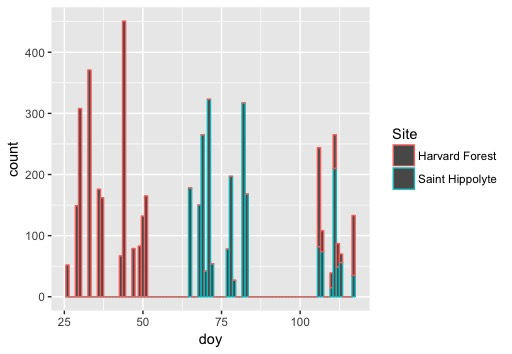
\includegraphics [scale=1.5]{measurement_day_hist.jpeg}[b]
\caption{Histogram of bud measurement dates for dataset 1}
\end{figure}
\newpage[h]

\section*{Feedback on feedback}
A)4\\
D)5\\
E)4\\

\end{document}
